\chapter{在室管理プラットフォーム\\「滞在ウォッチ」}\label{3}
本章では,ビーコンを用いた在室者検出および在室管理プラットフォーム「滞在ウォッチ」について述べる.
\ref{3.1}節では,「滞在ウォッチ」のシステム概要,利用した機器やサーバ,ビーコンと個人の紐付け,在室者推定,在室者管理サーバを述べる.
\ref{3.2}節では,在室者情報の活用方法として,現在の在室状況を示す在室者情報のリスト,過去の在室履歴を示す滞在時間や曜日別の滞在率による可視化を述べる.
\ref{3.3}節では,滞在ウォッチによって記録された入退室時刻の評価について述べる.
\ref{3.4}節では,滞在ウォッチによって記録された在室者情報を用いた応用システムについて述べる.




\section{「滞在ウォッチ」のシステム構成}\label{3.1}
% 本研究のシステム概要を図\ref{StayWatchOverview}に示す.
滞在ウォッチは,ビーコンを持ち歩き在室情報を記録するメンバ,メンバ管理,メンバへのビーコン配布,利用者の登録を行う管理者,現在状況や履歴を閲覧したりAPIを通して在室情報を利用する利用者(メンバや管理者も利用者になりうる),システムを開発する開発者がおり,メンバがビーコンを携帯し,部屋ごとに設置された受信機によりビーコンを検出する手法で,在室者管理を自動に行う.
メンバには一人1つビーコンを携帯してもらう.サーバには部屋メンバの名前とビーコンのIDを登録する.ビーコンは周囲に数秒に1回電波を発信する.
% 受信機がビーコンの電波を受信する間隔は3分である.
受信機が検出したビーコンのIDと電波強度は日時や在室した部屋名とともにサーバに送信され記録される.
記録した在室者情報はWeb APIを通して利用可能であり,勤怠管理システムや来訪促進システムといった様々な応用を想定している.

\begin{figure}[h]
  \centering  % 図を真ん中に配置
  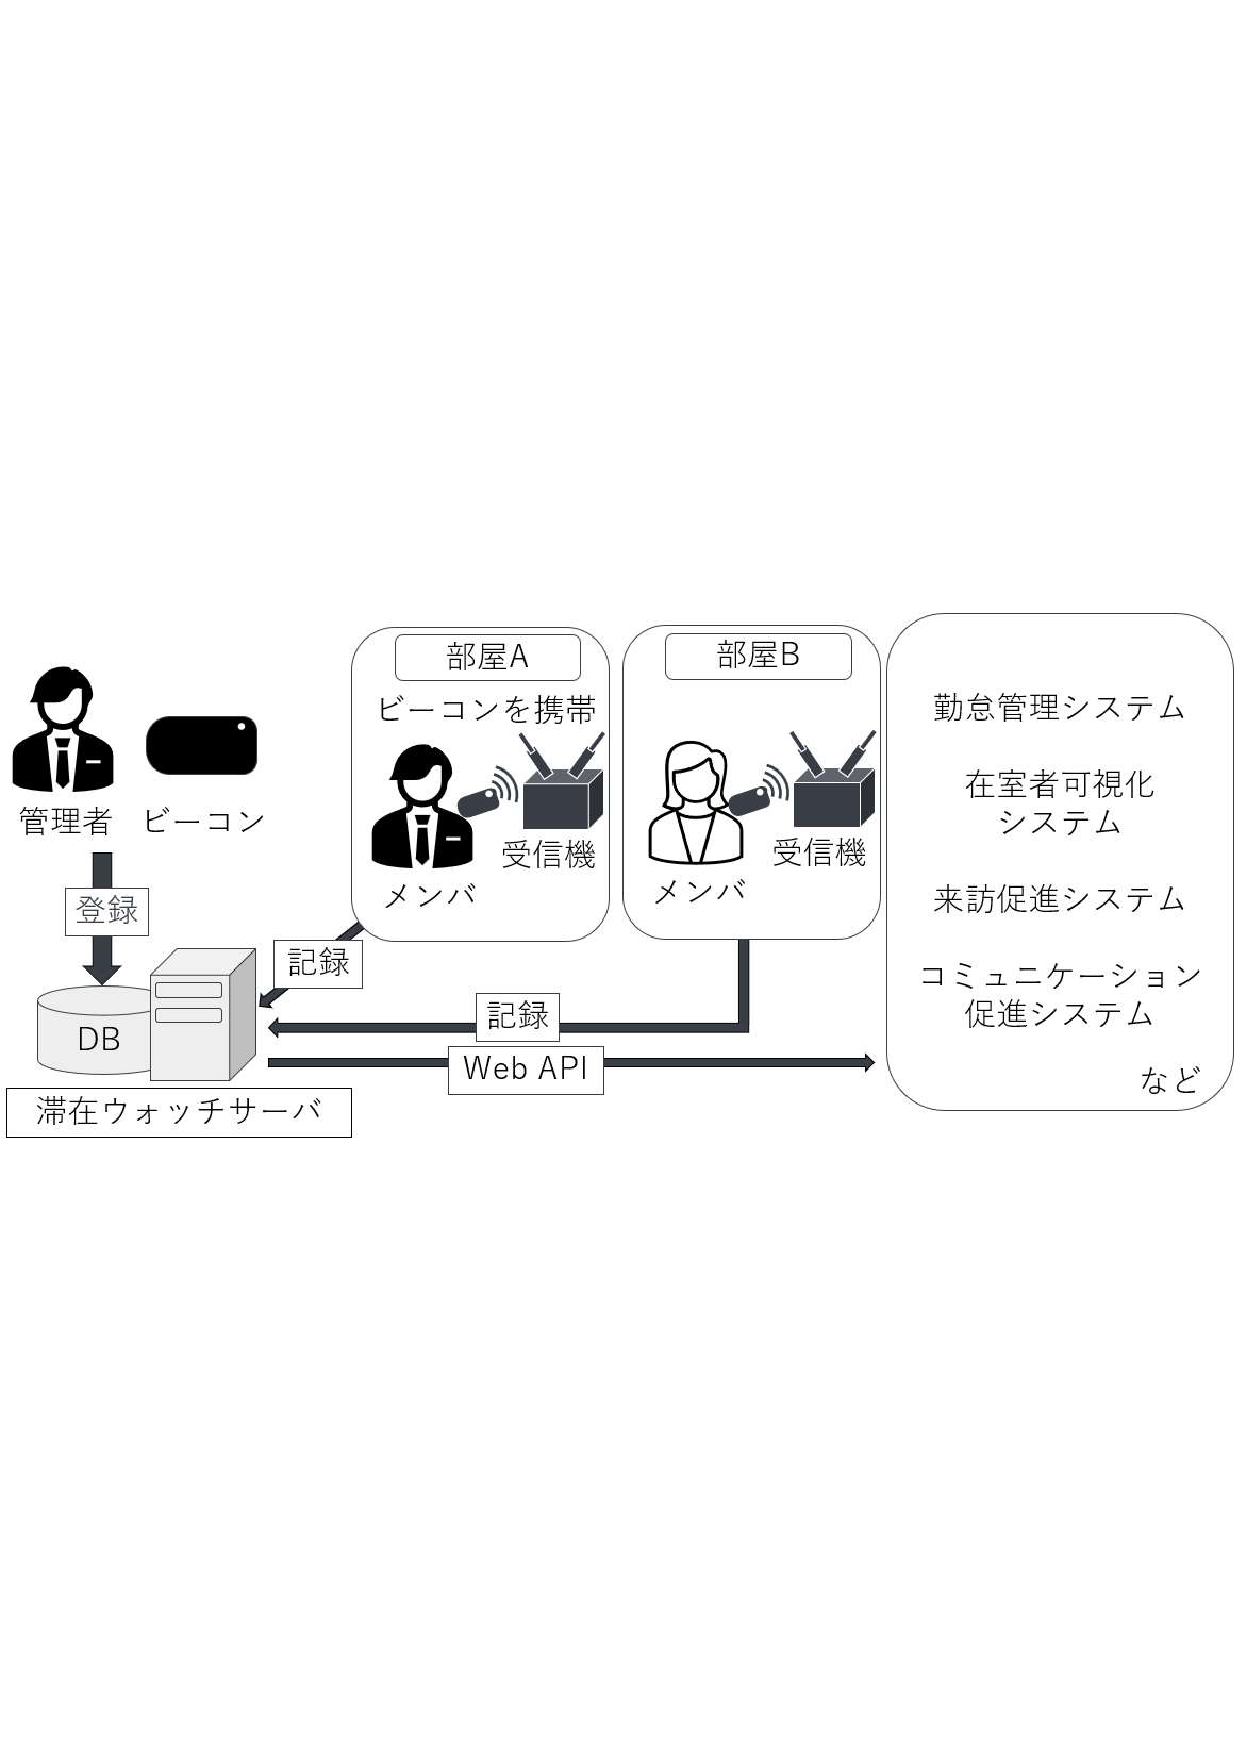
\includegraphics[clip,scale = 0.6]{image/system.pdf}
  \caption{「滞在ウォッチ」の概要図}    \label{StayWatchOverview}
\end{figure}

本手法に関連するビーコン,受信機,サーバを示す.
メンバが携帯するビーコンには,長期的な運用を考慮しバッテリ交換が可能かつ小型なFCS1301\cite{fcs1301}を利用している.
ビーコンは図\ref{fig:beacons}のように様々な大きさや形のものがある.
複数のビーコンの比較を表\ref{tb:beacons}に示す.
ボタンは定期的な電波発信に加えて押した時にも電波発信できるため,点検時に利用できる.
FCS1301の用途は,財布やパスケースなどの貴重品に付ける紛失防止や子供の荷物などに付ける見守り支援がある.
% 実際にパスケースに取り付けた様子を図\ref{fig:beaconforpass}に示す.
財布やパスケースに取り付けたり入れられるサイズである.
そのため,メンバが携帯するのに適している.
またバッテリ交換の際の様子を図\ref{fig:batchange}に示す.
特殊な器具などを使う必要がなく,簡単にバッテリ交換ができる.
FCS1301ではボタンを押すとペアリング,長押しするとスリープモードへ移行し,保管の間省電力モードになる.
ビーコンの電波送信の間隔はFCS1301の規格で最大の10秒ごとに設定している.
1部屋ごとに台設置する受信機には図\ref{fig:raspi} の低価格な Raspberry Pi\cite{raspi} を利用している.
1つの部屋に1つずつ受信機を設置する.
% サーバには,Google Cloud Platform\cite{gcp}を利用している.

\begin{figure}[H]
  \begin{center}
    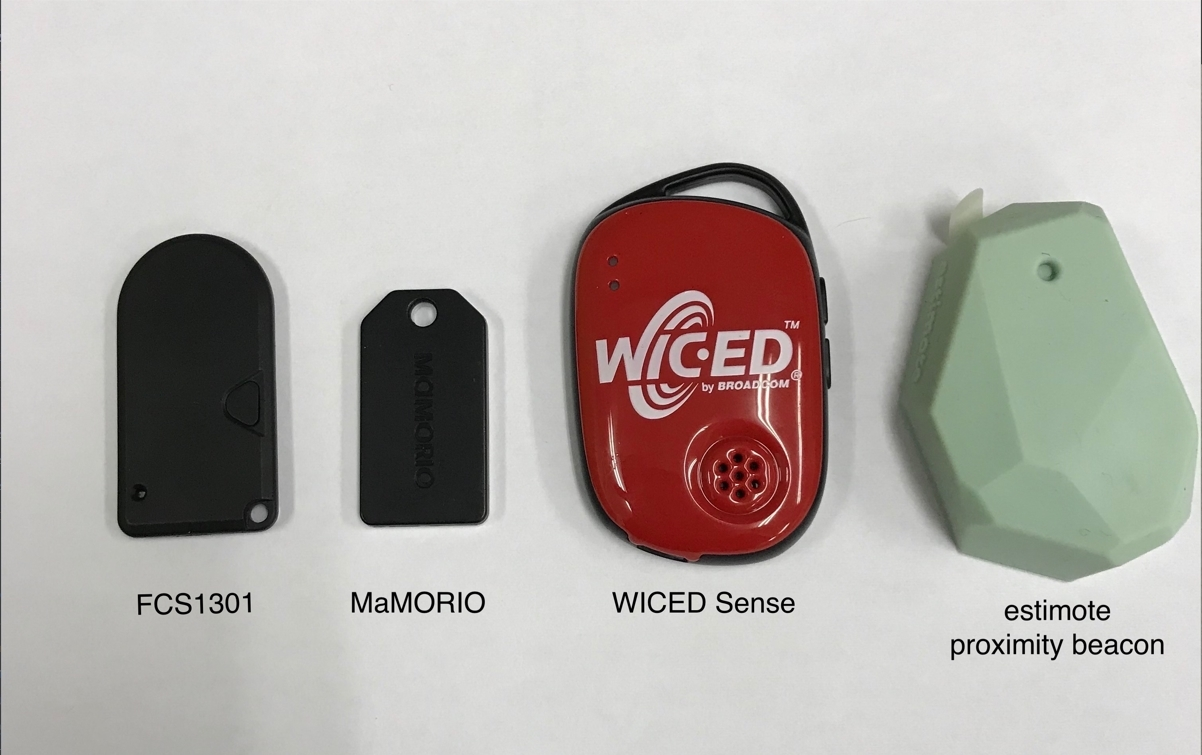
\includegraphics[width=150mm]{image/beaconType.jpg}
    \caption{ビーコンの種類}
    \label{fig:beacons}
  \end{center}
\end{figure}

\begin{table}[H]
  \begin{center}
    \caption{ビーコンの比較}
    \label{tb:beacons}
    \begin{tabular}{|l|c|c|c|} \hline
      ビーコン名    & サイズ                           & バッテリ交換 & ボタン \\ \hline \hline
      FCS1301  & 縦46.0 mm× 横24.5 mm× 厚さ3.5 mm  & ○      & ○   \\
      MAMORIO  & 縦35.5 mm× 横19.0 mm× 厚さ3.4 mm  & ×      & ×   \\
      WICED    & 縦60.0 mm× 横37.0 mm× 厚さ10.0 mm & ○      & ○   \\
      estimote & 縦55.0 mm× 横38.0 mm× 厚さ15.0 mm & ×      & ×   \\\hline
    \end{tabular}
  \end{center}
\end{table}

% \begin{figure}[H]
%   \begin{center}
%     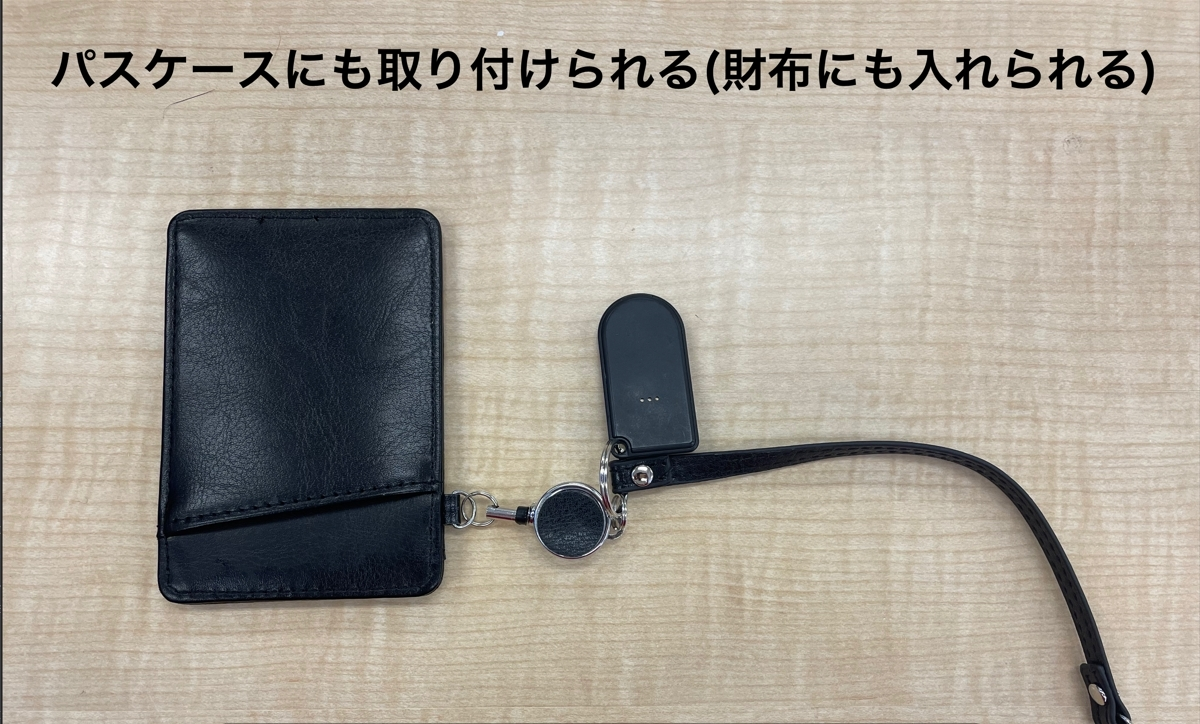
\includegraphics[width=150mm]{image/beaconForpass.jpg}
%     \caption{パスケースに取り付けたビーコン}
%     \label{fig:beaconforpass}
%   \end{center}
% \end{figure}

\begin{figure}[H]
  \begin{center}
    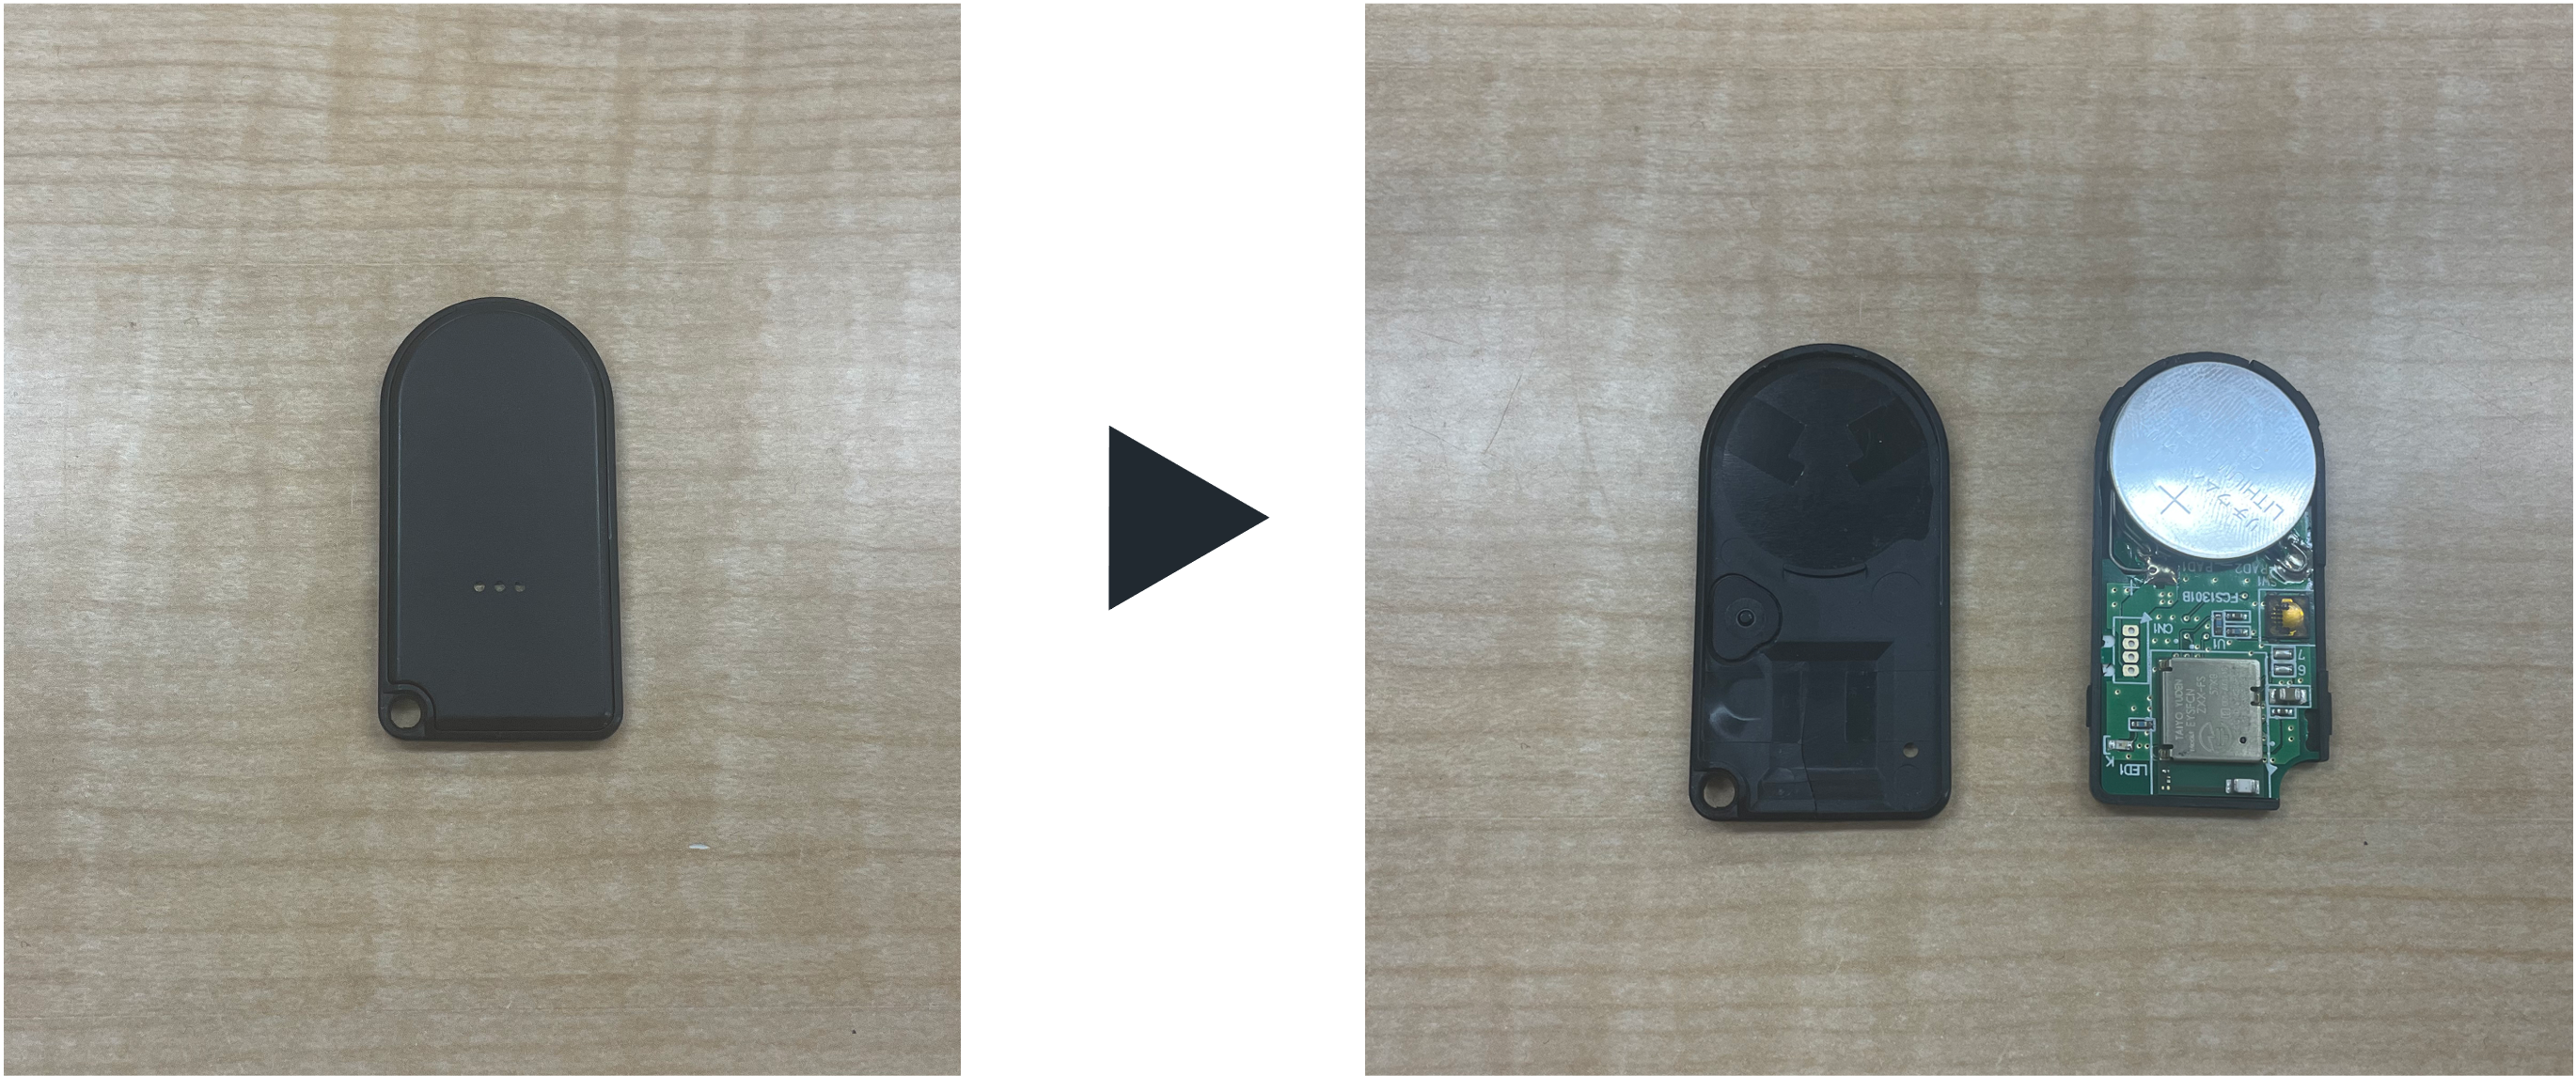
\includegraphics[width=150mm]{image/batchange.png}
    \caption{ビーコンのバッテリ交換}
    \label{fig:batchange}
  \end{center}
\end{figure}

\begin{figure}[H]
  \begin{center}
    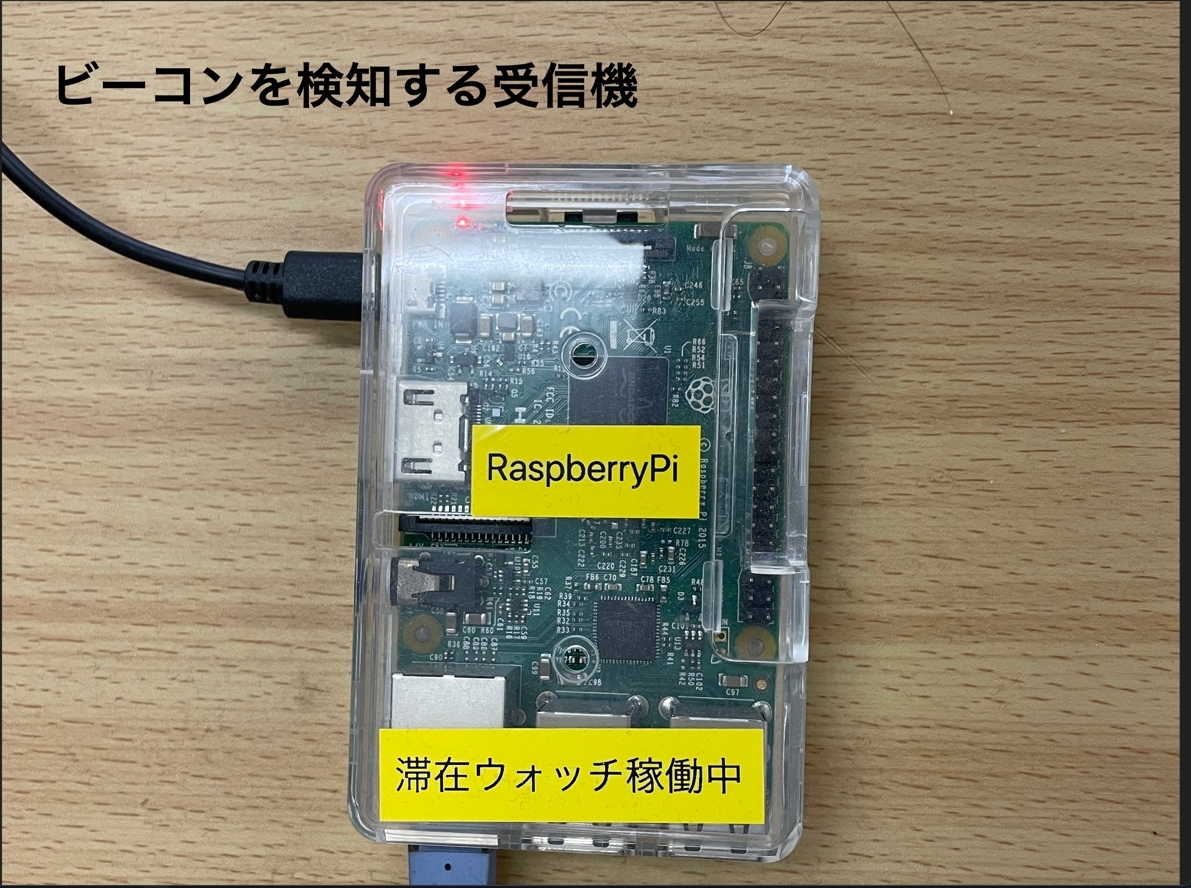
\includegraphics[width=150mm]{image/RasPi.jpg}
    \caption{実際に使用しているビーコンを検知する受信機}
    \label{fig:raspi}
  \end{center}
\end{figure}

% 個人を特定する在室者の検出手法には,個人と在室者情報を紐付けする必要がある.
% ビーコンを用いた検出手法ではビーコンのIDとメンバの名前をサーバのデータベースに登録している.
% 登録には図\ref{fig:ent}のウェブサイトを用いて行う.
% グループ分けとして研究室やチームの属性を追加している.
% これは可視化において個人の識別を容易にし,来訪促進システムでは連帯感や競争心を刺激でき,ゲーミフィケーション\cite{gamification}を取り入れる上で有用な情報だと考えている.
% UUID,major,minorはビーコン固有の識別子であり,先述のビーコンのIDに該当する.

% \begin{figure}[H]
%   \begin{center}
%     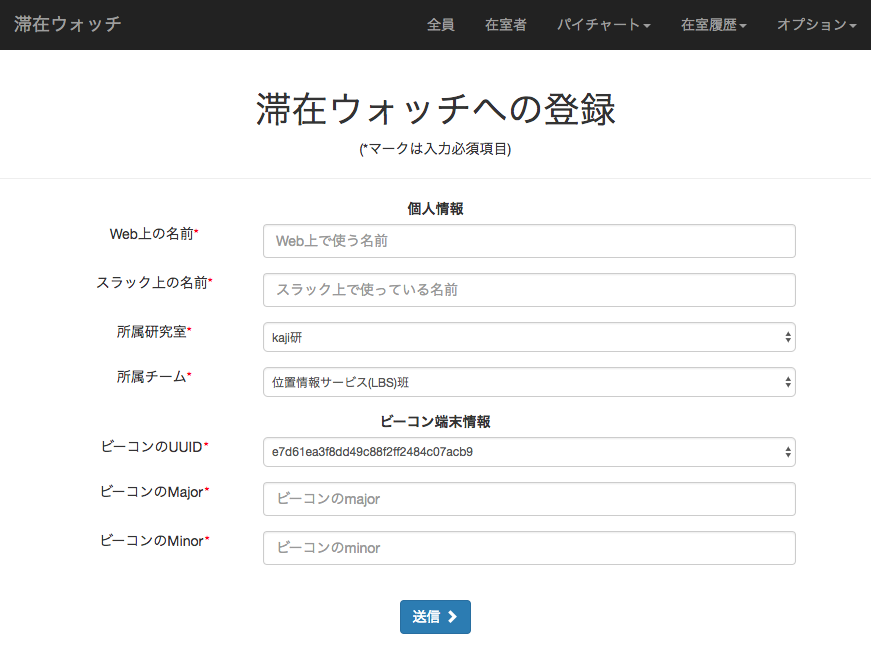
\includegraphics[width=160mm]{image/RegistrationScreen.png}
%     \caption{登録画面}
%     \label{fig:ent}
%   \end{center}
% \end{figure}

メンバがビーコンを携帯し部屋に訪れると,部屋ごとに設置された受信機でビーコンを検出する.
この手法では,メンバは常にビーコンを所持している必要がある.
FCS1301は小型で薄いビーコンのため,財布の中や鍵のキーホルダーとして貴重品などと一緒に持ち歩ける.
この手法では,一時的に部屋を出た場合にも在室判定ができ,メンバはビーコンを所持するだけで,在室者情報を記録できる.
メンバが部屋を訪れた際,部屋ごとに設置された受信機で検出されたビーコンの情報とサーバにある登録情報を参照し,在室者を特定する.
また,複数の部屋に受信機を設置するため,在室者の名前に加えて部屋名もサーバに送信する.
部屋ごとに受信機を設置する際に,設置する部屋が隣接する場合に以下の問題が発生する可能性がある.
ビーコンは周囲数メートルから数十メートルに電波を発信するため,隣接した複数の部屋で同様の在室判定を行う可能性がある.
そこで,ビーコンが発信する電波強度に着目する.
ビーコンの電波強度は表\ref{tb:rf}に示すように壁や扉のコンクリートや鉄板の障害物によって減衰する\cite{barrier}.
そのため,隣接した複数の部屋では電波強度に明らかな差があると考えられる.
受信機から送られてきた電波強度を比較すれば,正確な在室判定が可能である.
したがって,在室判定にビーコンの受信電波強度を利用して隣接した部屋での誤検出の防止が可能だと考える.
部屋ごとに設置された受信機によって検出された在室者情報はサーバに送られ,データベースに日時と在室した部屋名が記録される.
記録した在室者情報はWeb APIを通して利用可能であり,他のプログラムからも利用できる.

\begin{table}[H]
  \begin{center}
    \caption{高周波 (RF) 電波を反射/吸収する物質}
    \label{tb:rf}
    \begin{tabular}{|c||c|c|c|c|c|c|c|c|c|} \hline
      障壁の種類  & 木材 & 合成物質 & ガラス & 水 & 煉瓦 & 大理石 & 土壁 & コンクリート & 金属    \\ \hline
      干渉の可能性 & 低  & 低    & 低   & 中 & 中  & 中   & 高  & 高      & 非常に高い \\ \hline
    \end{tabular}
  \end{center}
\end{table}


% Web APIの利用方法は指定のURLを開くとJSON形式\cite{json}で取得できる.
% 例えば,https://kajilab.net/stay-watch/stay にアクセスすると現在の在室者情報が取得できる.
% 実際に取得したJSON形式の在室者情報を図\ref{jsonstay}に示す.
% 図\ref{jsonstay}に示すように,現在在室している人のID,名前,所属,在室している部屋を取得できる.
% この他にもhttps://kajilab.net/stay-watch/ に続けてリクエストパラメータがある.
% リクエストパラメータについて表\ref{request}に示す.

% \begin{figure}[H]
%   \begin{center}
%     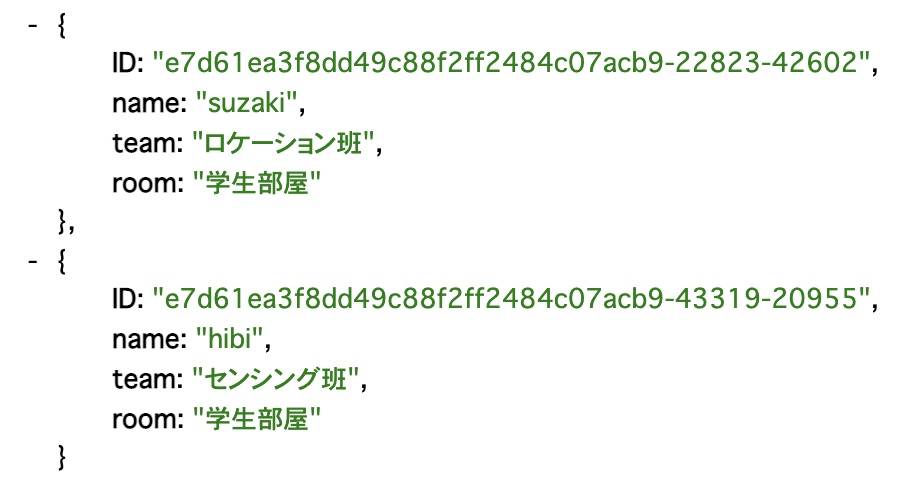
\includegraphics[width=160mm]{image/jsonstay.png}
%     \caption{JSON形式で取得した現在の在室者情報}
%     \label{jsonstay}
%   \end{center}
% \end{figure}
% \begin{table}[H]
%   \begin{center}
%     \caption{リクエストパラメータ一覧}
%     \label{request}
%     \begin{tabular}{|l|c|c|} \hline
%       パラメータ             & 値     & 説明                                       \\ \hline
%       stay                   & string & 現在の在室者を取得する                     \\ \hline
%       log                    & string & 今日の在室情報のみを取得する               \\ \hline
%       log?date1= YYYY-MM-DD
%                              & string & 過去の在室情報を取得(date1からdate2)       \\

%       \&date2=MMMM-YY-DD     &        &                                            \\\hline
%       last-time              & string & 最後に滞在を確認できた時間を取得する       \\ \hline
%       log-time               & string & 過去の累計滞在時間を取得する               \\ \hline
%       log-time?month=YYYY-MM & string & 過去の累計滞在時間を月ごとに取得する       \\ \hline
%       log-group              & stirng & その日だけのグループの滞在情報を取得する   \\ \hline
%       log-group?date1=YYYY-MM-DD
%                              & stirng & 期間を指定してグループの滞在情報を取得する \\
%       \&date2=YYYY-MM-DD     &        & (date1からdate2)                           \\\hline
%     \end{tabular}
%   \end{center}
% \end{table}
\section{在室者情報の可視化}\label{3.2}
研究室やコワーキングスペースでは「今,誰がどこにいるのか」といった情報の共有が行われている.
これは利用者において目的とする人の居場所が把握できれば,接触までのアプローチが容易になり,コミュニケーションの円滑化や共同作業を支援できる.
管理者においても部屋の利用者数や時間帯が把握できれば,室内の温度調整を始めとする環境整備や活用状況が少ない部屋の省エネ化の指標となる.
この在室者情報を確認できるように図\ref{fig:list}のリストを構築している.
会いたい人の居場所を知るには,本人を探す,本人に連絡して聞く,事前に聞くといったアプローチが必要にある.
本人を探す場合は,部屋が複数あったり,離れていたりするとそれは困難になる.
本人に連絡して聞く場合は相手の状況,連絡手段によって,現在の情報を取得するには時間的な制限がある.
事前に聞く場合,両者は時間的な拘束を受けており,いつでもコミュニケーションが取れるとは限らない.
そのため,在室情報を何らかの方法で知れると,相手を介した居場所の確認の必要がなくなる.
そこで,教員が部屋に在室しているかが外から把握できるように,図\ref{fig:monitor}に示すような教員の在室状況モニタを試験運用としてドアに設置した.
この試験モニタによって,教員に部屋に在室しているか聞く必要がなくなり,アプローチしやすくなると考える.
% \begin{figure}[H]
%   \begin{center}
%     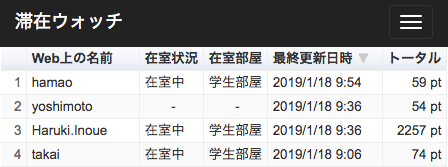
\includegraphics[width=150mm]{image/ListOccupancy.png}
%     \caption{在室情報のリスト}
%     \label{fig:list}
%   \end{center}
% \end{figure}

% \begin{figure}[H]
%   \begin{center}
%     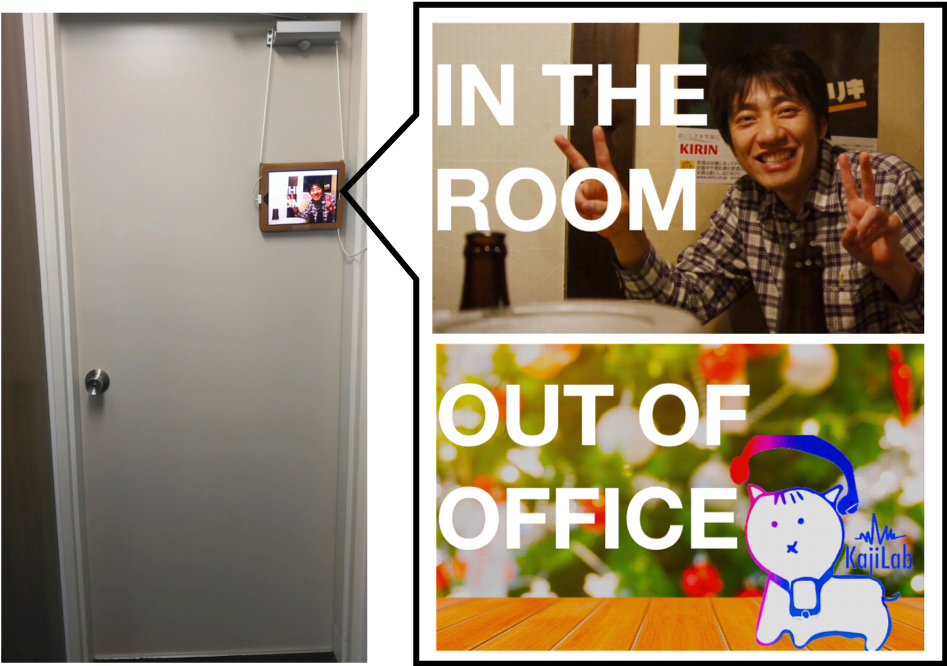
\includegraphics[width=150mm]{image/OccupancyMonitor.png}
%     \caption{教員の在室状況モニタ}
%     \label{fig:monitor}
%   \end{center}
% \end{figure}

過去の在室状況からは利用者が人の訪問場所の傾向が把握できるため,次の人の訪問場所の予測がある程度可能である.
これにより,円滑なコミュニケーションの補助になると考える.
例えば,相手に会う約束をするほどではないが,一緒に作業をしたら効率が良くなるといった場合が該当する.
管理者は部屋の利用状況を把握でき,室内の温度調整を始めとする環境整備や活用状況が少ない部屋の省エネ化の指標となる.
そこで過去の在室履歴を図\ref{fig:staytime}の滞在時間,図\ref{fig:weekday}の曜日別の滞在率,図\ref{fig:group}の班別の滞在率,図\ref{fig:total}の合計滞在時間をグラフで示している.

% \begin{figure}[H]
%   \begin{center}
%     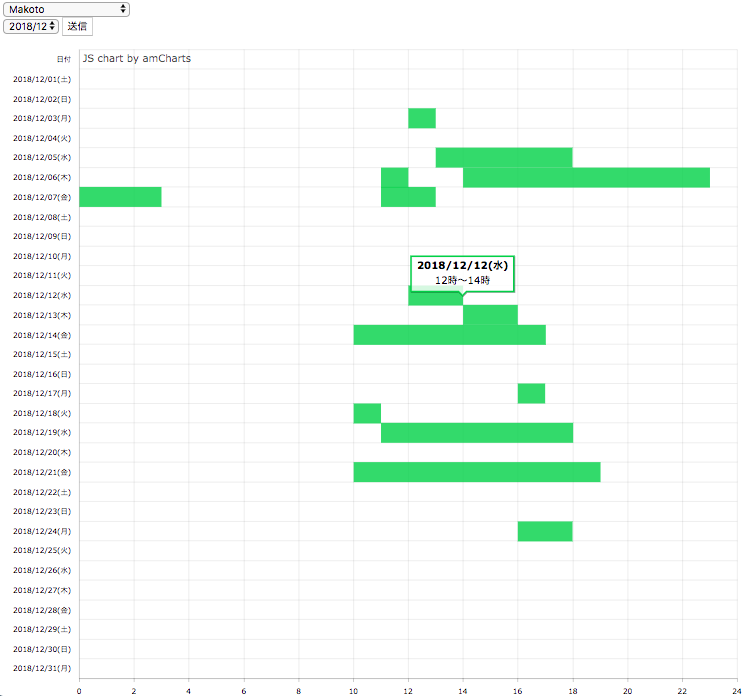
\includegraphics[width=160mm]{image/StayTime.png}
%     \caption{滞在時間のグラフ}
%     \label{fig:staytime}
%   \end{center}
% \end{figure}

% \begin{figure}[H]
%   \begin{center}
%     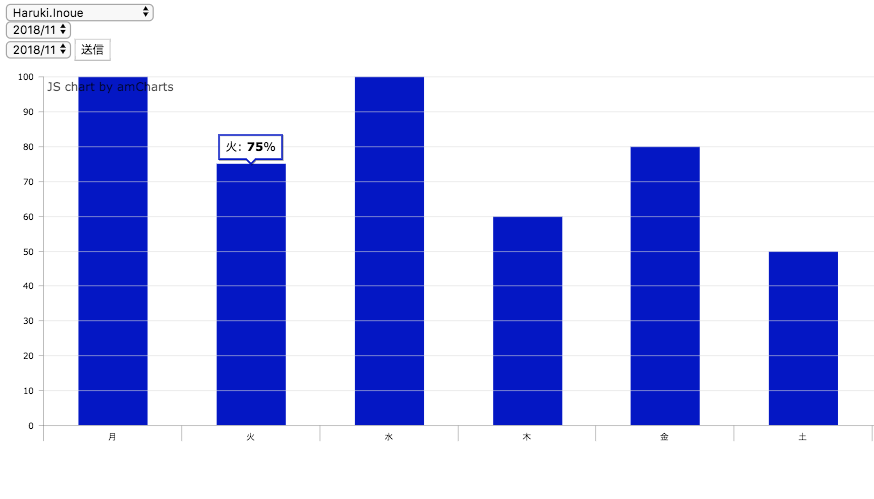
\includegraphics[width=160mm]{image/StayRateWeek.png}
%     \caption{曜日別の滞在率のグラフ}
%     \label{fig:weekday}
%   \end{center}
% \end{figure}

% \begin{figure}[H]
%   \begin{center}
%     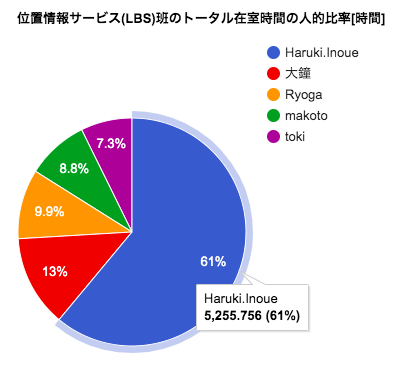
\includegraphics[width=150mm]{image/StayRateGroup.png}
%     \caption{班別の滞在率のグラフ}
%     \label{fig:group}
%   \end{center}
% \end{figure}

% \begin{figure}[H]
%   \begin{center}
%     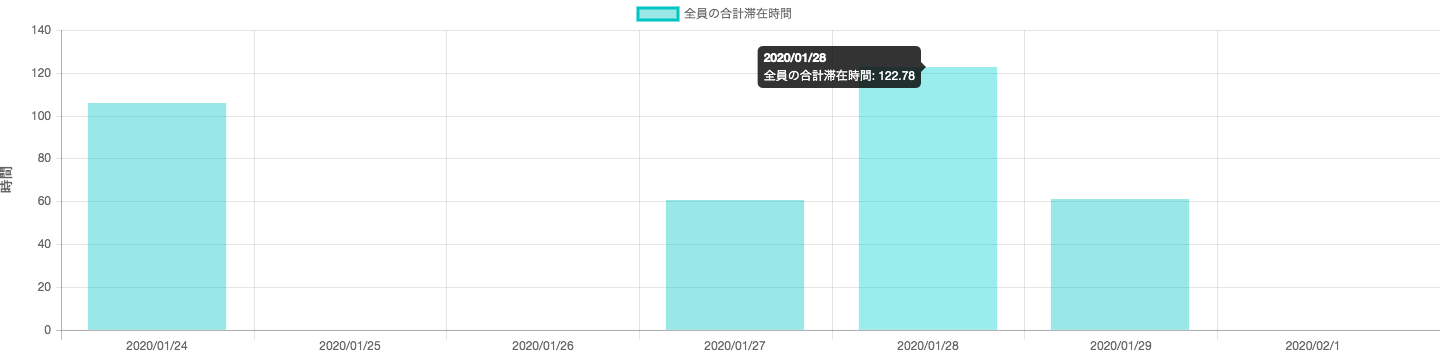
\includegraphics[width=160mm]{image/TotalStayTime.png}
%     \caption{合計滞在時間のグラフ}
%     \label{fig:total}
%   \end{center}
% \end{figure}









\section{部屋利用者の入退室時刻の評価実験}\label{3.3}
滞在ウォッチで記録された部屋利用者の入退室時刻が正確に記録されているか,ビーコンが電池切れをせずに記録されているかを確認するための評価実験を行う.
滞在ウォッチのシステム構成でも説明した通り,受信機がビーコンの電波を受信する間隔は3分である.
そのため,滞在ウォッチで記録される入退室時刻は実際に入退室した時刻と比べて誤差が3分以内であるのが望ましい.
また在室管理プラットフォームであるため,来訪した部屋利用者全員の在室者情報が記録されてなければいけない.
電池切れをせずに正確に記録されているか,電池切れをしている利用者がどの程度存在するのかを確認する.

本研究で使用しているビーコンは,電池で動作しているため,電池切れの際は電池交換をする必要がある.
電池が切れていると在室者情報は記録できないため,ビーコンの電池が切れているかどうかを通知する必要がある.
通知をする手段としてSlackでの通知を行う.
実際に電池切れを通知した際の様子を図\ref{batoff}に示す.
Slackでの通知を行う理由として,研究室に所属する人全員がSlackを通して連絡やコミュニケーションをとっているからである.
電池切れ通知は,5日以上受信機がビーコンの電波を検知できない人にする.
5日以上の理由として,本研究室では火曜日と金曜日にミーティングが行われるため,5日以上間隔が開く場合は電池切れの可能性が高いからである.
しかし図\ref{batoff}のように,100日以上検知できていないにも関わらず,電池交換がされていない利用者がいる.
電池交換をしていない利用者の特徴として,研究室にこないため電池交換をそもそもしない,通知が来ても電池交換が面倒でそのままにするのが挙げられる.
そのため電池切れの通知だけでは電池交換を行ってくれない可能性がある.
また,Slackでの通知のみでは利用者がメッセージの重要度を低く見積もる可能性があるため,管理者からも利用者に対し適宜コンタクトを取る必要があると考える.
電池切れの通知による電池交換の実行率や完了率を増やすには,改善点として通知頻度の見直しが挙げられる.

\begin{figure}[H]
  \begin{center}
    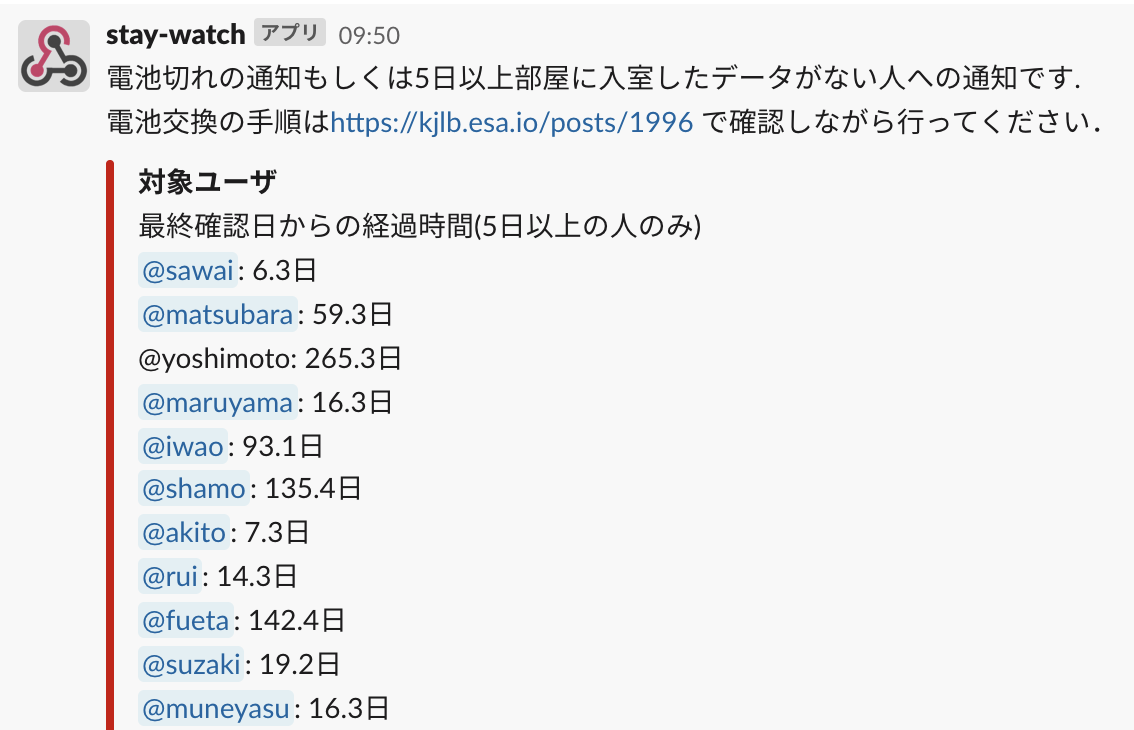
\includegraphics[width=160mm]{image/batoff.png}
    \caption{Slackによる電池切れ通知の実際の様子}
    \label{batoff}
  \end{center}
\end{figure}

2022年1月11日に入退室した13人の部屋利用者と時刻をビデオで撮影し,実際に入退室した時刻と滞在ウォッチで記録された時刻を比較する.
比較した結果を表\ref{actualTimeEstimationTime},表\ref{actualTimeEstimationTime2}に示す.
比較結果として入室時刻の平均誤差が1分.退室時刻の平均誤差が2分であった.
3分毎に受信機がビーコンの電波を検知するので,3分以内の誤差であれば十分な精度であると考える.
しかし,来訪したにも関わらず,記録されていない利用者もいた.
今回在室者情報が記録された利用者は13人,記録できなかった利用者は7人であった.
つまり,記録できなかった利用者は電池切れの通知をしても電池交換をしなかったと考えられる.
今後の課題として,在室者情報が記録できなかった利用者に対してアンケートを行い,なぜ電池交換をしないのか,どのような電池切れ通知するべきか,通知方法,通知頻度を聞く必要がある.
\begin{table}[H]
  \centering
  \caption{実際の入退室時刻と滞在ウォッチで記録された時刻の比較}
  \label{actualTimeEstimationTime}
  \begin{tabular}{|c|c|c|}
    \hline
            & 実際に入退室した時刻   & 滞在ウォッチで記録された     \\
            &                        & 入退室時刻                   \\
    \hline
            & 入室時刻 退室時刻      & 入室時刻\hspace{5mm}退室時刻 \\
    \hline
    利用者A & 09:01\hspace{7mm}10:51 & 09:03:15\hspace{6mm}10:53:13 \\
    利用者B & 08:43\hspace{7mm}10:27 & 08:44:56\hspace{6mm}10:31:50 \\
    利用者C & 08:25\hspace{7mm}10:27 & 08:26:37\hspace{6mm}10:31:50 \\
    利用者D & 10:20\hspace{7mm}19:43 & 10:22:40\hspace{6mm}19:46:05 \\
    利用者E & 10:46\hspace{7mm}14:51 & 10:47:06\hspace{6mm}14:53:59 \\
    利用者F & 10:43\hspace{7mm}13:31 & 10:44:03\hspace{6mm}13:34:54 \\
    利用者G & 10:46\hspace{7mm}15:30 & 10:47:06\hspace{6mm}15:33:30 \\
    利用者H & 10:52\hspace{7mm}12:43 & 10:53:13\hspace{6mm}12:46:12 \\
    利用者I & 10:25\hspace{7mm}14:40 & 10:25:43\hspace{6mm}14:41:48 \\
    利用者J & 10:05\hspace{7mm}15:26 & 10:07:24\hspace{6mm}15:30:28 \\
    利用者K & 12:05\hspace{7mm}18:25 & 12:06:30\hspace{6mm}18:26:58 \\
    利用者L & 10:28\hspace{7mm}14:29 & 10:28:46\hspace{6mm}14:32:41 \\
    利用者M & 12:05\hspace{7mm}17:26 & 12:06:30\hspace{6mm}17:29:11 \\
    \hline
  \end{tabular}
\end{table}
\begin{table}[H]
  \centering
  \caption{実際の入退室時刻と「滞在ウォッチ」で記録された時刻の平均絶対誤差}
  \label{actualTimeEstimationTime2}
  \begin{tabular}{|c|c|}
    \hline
    入室した時刻の平均絶対誤差 & 退室した時刻の平均絶対誤差 \\
    \hline
    1分                        & 2分                        \\
    \hline
  \end{tabular}
\end{table}

\section{在室者情報を用いた応用システムについて}\label{3.4}
部屋利用するメンバの在室者情報を用いれば,部屋の管理者や利用者にとって便利な応用システムが考えられる.
1つ目の応用システムとして,勤怠管理システムが考えられる.
勤怠管理システムの代表例としてタイムカードでの打刻や,ICカードやQRコード,スマートフォンによる記録が挙げられる.
これらのシステムでは利用者が能動的に記録する必要がある.
本研究でのビーコンを用いた手法では能動的な記録を必要とせず,自動で記録されるため,利用者の負担や記録忘れが減ると考えられる.

2つ目の応用システムとして,コミュニケーション機会の損失を減らすシステムが考えられる.
% 研究室では在室中に特定の人物がいつ来るかを
研究室では利用者同士の活発なコミュニケーションが求められる.
しかし研究室内で目的とする人物と直接会うのを希望していたとしても,その人物が来るかどうかはその人にとって不明である.
会うのを希望する人に対してSNSなどのコミュニケーションツールを使っていつ頃くるかと言った連絡を取ることもできるが,仲が良い人でないとメッセージのやり取りに心理的なハードルが存在する.
そこでこれを改善する既存研究として図\ref{petgaiyou}に示す「今日の滞在」というシステムがある.
% そこで部屋利用者が共有できる情報である在室者情報を用いてコミュニケーションを促進するようなシステムがある.
このシステムでは普段の在室者の入退室情報を用いて,来そう,帰りそうという状態を予測し,その予測結果と実際の部屋の在室者と退室者の状態を提示するシステムである.
この情報をWebサイトと研究室内のディスプレイに表示し,来そう,帰りそうという表示をもとにコミュニケーション機会の損失を軽減するのが目的である.
% コミュニケーション促進システムについては4章で実装した「きょうの滞在」で詳しく述べる.

3つ目の応用システムとして,来訪促進システムが考えられる.
在室者情報を用いたゲーミフィケーションに基づくシステムが考えられる.
具体例として在室履歴を用いたペット育成ゲームが考えられる.
在室履歴を用いたペット育成ゲームの概要を図\ref{petgaiyou}に示す.
部屋利用者の在室履歴からペットに餌を与えられるようなシステムである.
部屋利用者はペットに餌を与えるためには部屋に在室する必要がある.
そのためペットに愛着があるなら部屋利用者は来訪する必要がありこれによって来訪促進が期待できる.
% また在室履歴を用いたペット育成ゲームのアプリのイメージ図を図\ref{petimage}に示す.
% 誰でも見やすいようなレイアウトやスマホでの利用を想定したボタン配置を意識した.
\begin{figure}[H]
  \begin{center}
    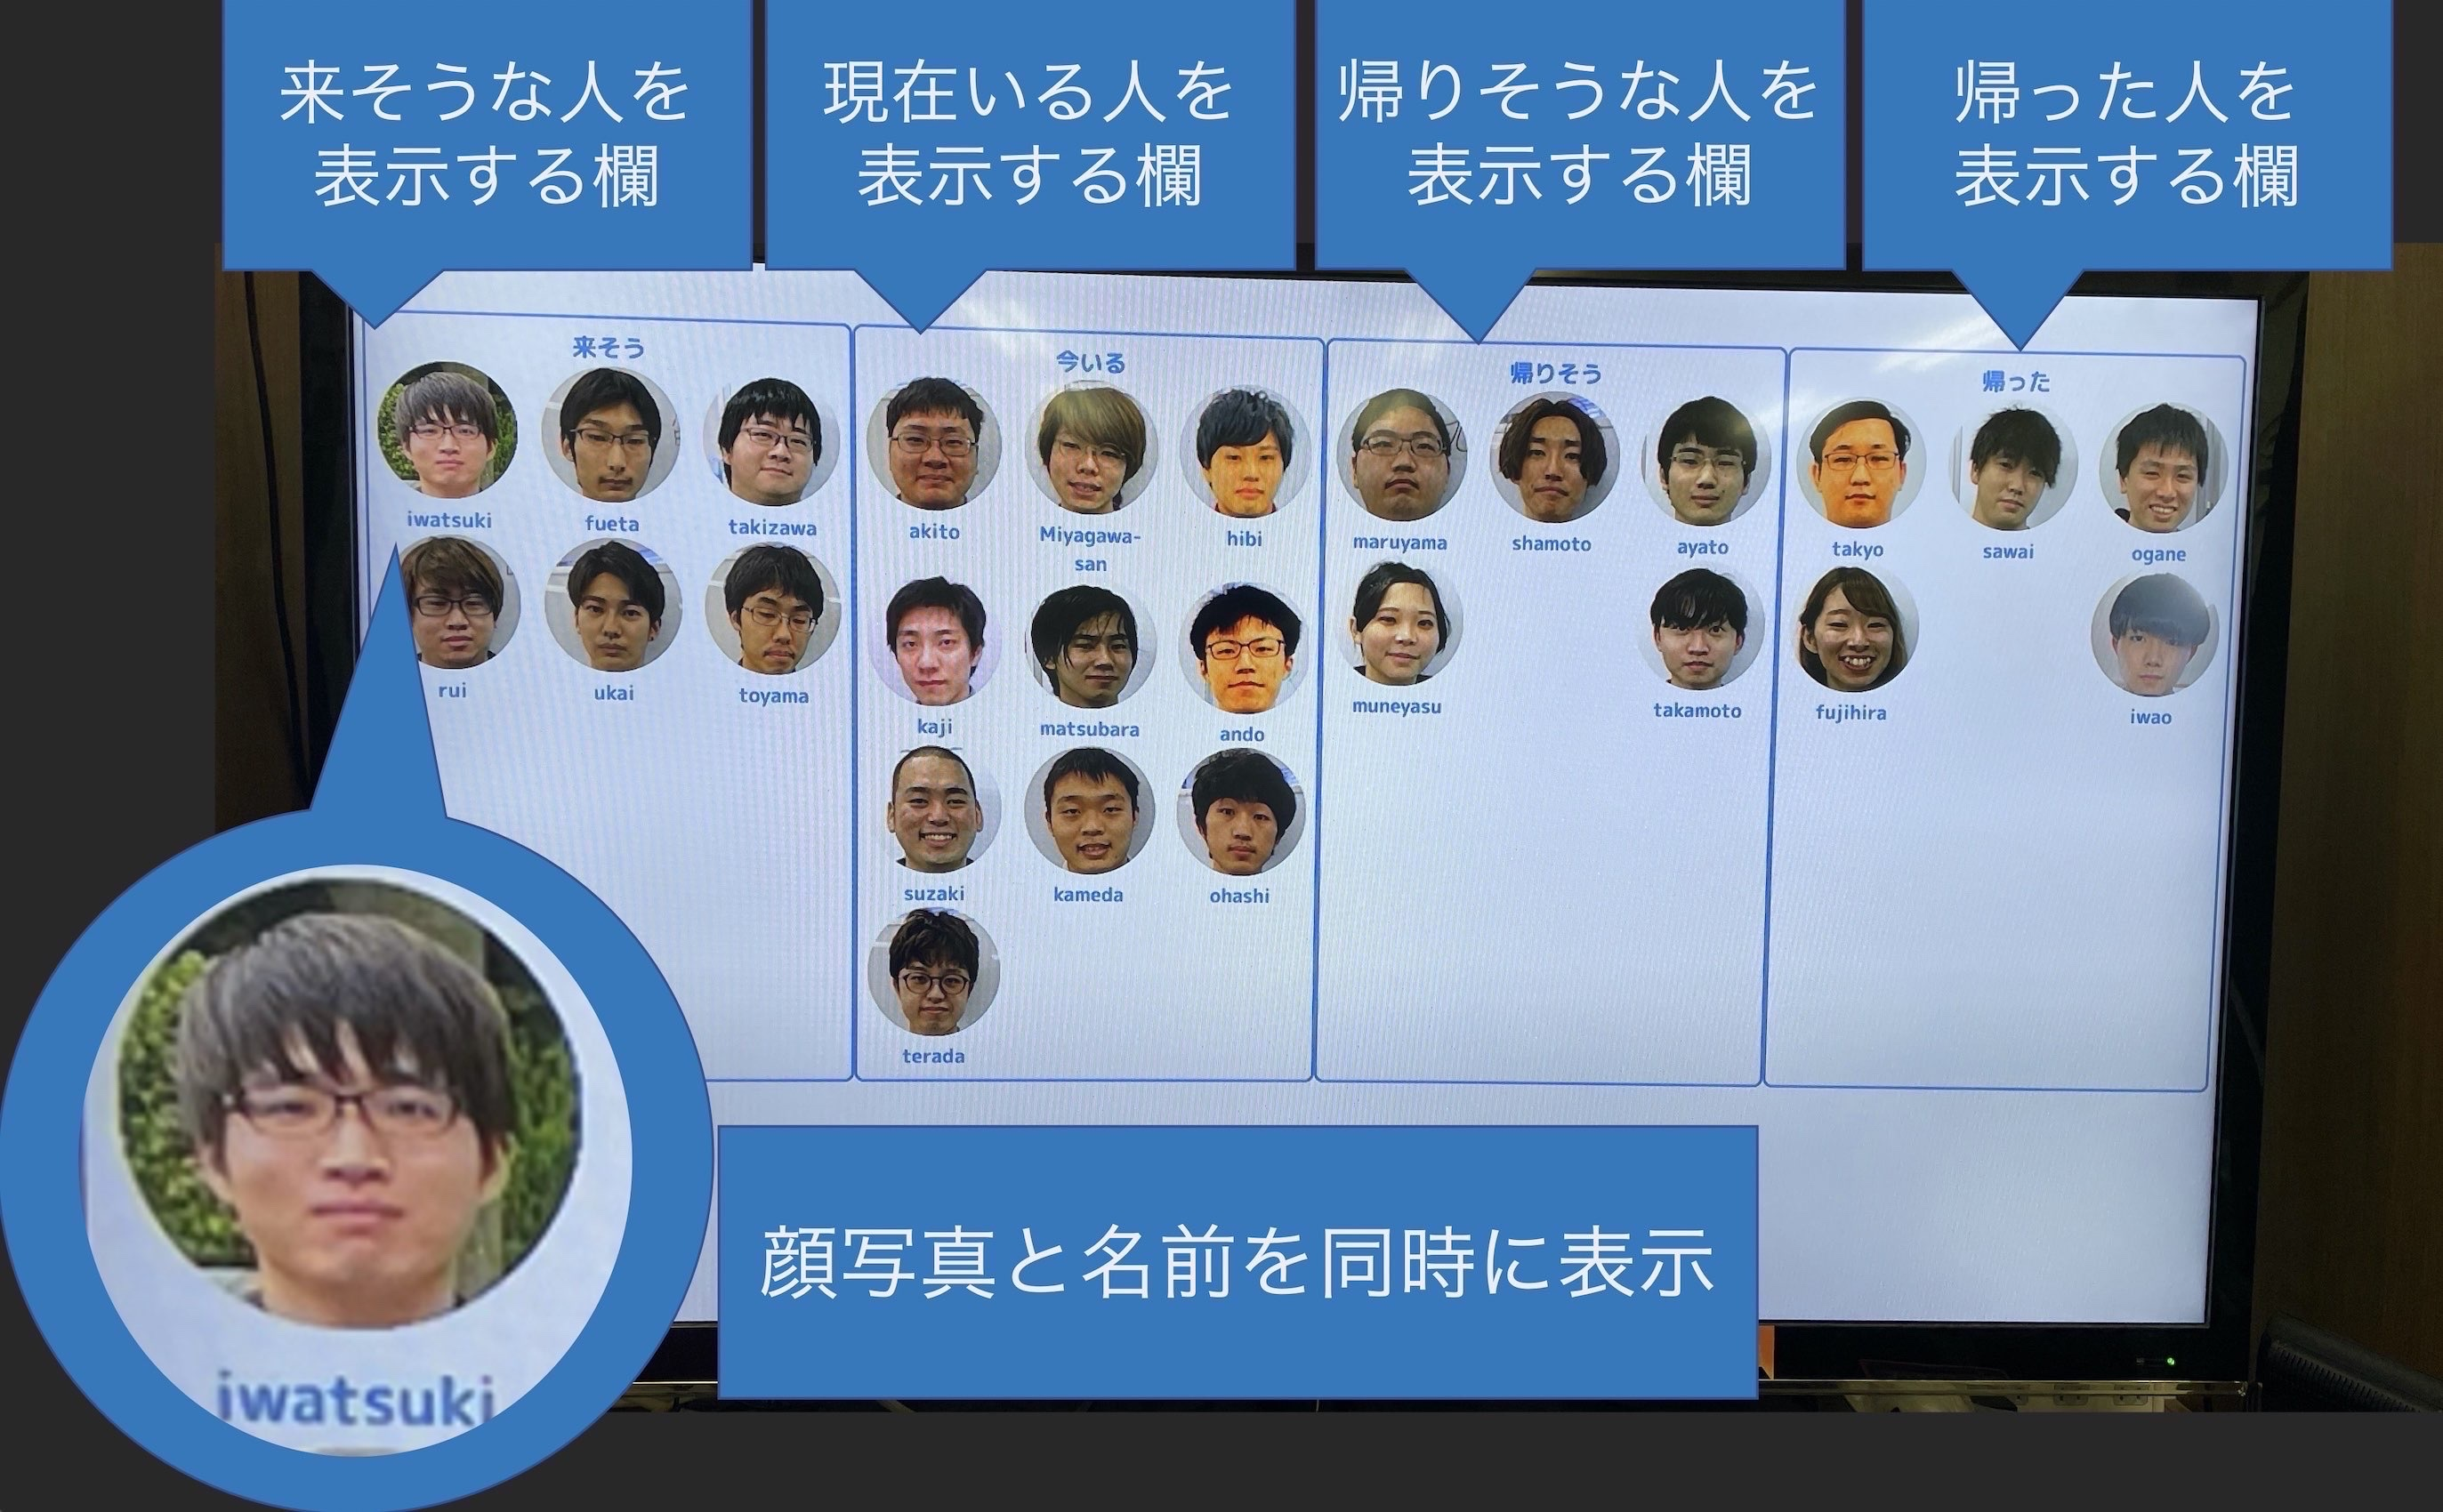
\includegraphics[width=160mm]{image/todayStay.jpg}
    \caption{コミュニケーション機会の損失を減らすシステム}
    \label{todayStay}
  \end{center}
\end{figure}

\begin{figure}[H]
  \begin{center}
    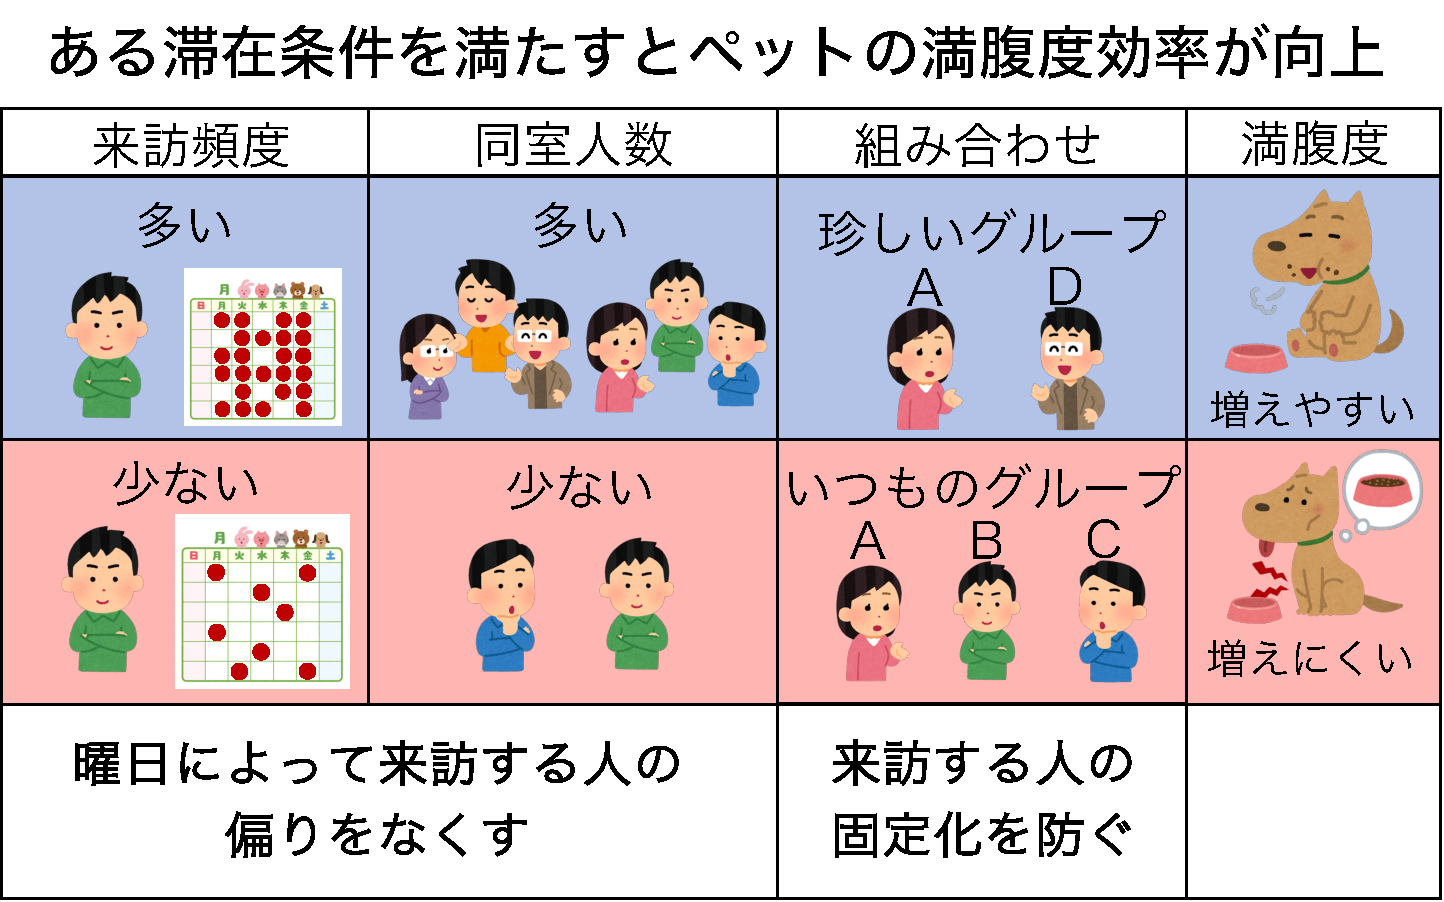
\includegraphics[width=160mm]{image/petgaiyou.pdf}
    \caption{ペット育成ゲームのアプリのイメージ}
    \label{petgaiyou}
  \end{center}
\end{figure}

\thispagestyle{myheadings}
